\chapter{Audio Scene Analysis meets Signal Processing}\label{ch:application}

\newthought{Synopsis} \synopsisChApplication

\mynewline
Here, we presents some audio scene analysis problems that will be later discussed in their echo-aware extension.
Following the last part's structure, this introductory chapter gathers the common knowledge shared across the following ones.
Here we make a strong transition: we assume the echo properties are known a priori, so that the our focus is on the benefit of their knowledge.
The literature for each of them is reviewed, but since it is vast and spans diverse scientific research decades, we do not aim to cover it entirely.
Moreover, since the following chapters are dedicated to each of these problems under the echo-aware perspective, this specific literature is not considered here.
\\The material presented here results from the personal synthesis of concepts and references available in the literature.
Furthermore, some definitions are digested from classical textbooks already used for this thesis, such as~\citeonly{vincent2018audio}.

\section{Audio Scene Analysis Problems}\label{sec:application:scenario}
As mentioned in the first chapter, audio scene analysis aims to extract relevant information in the audio scene.
Different types of information are estimated or inferred by solving specific problems.
Despite their diversity, most of these problems can be defined with a common model.

\subsection{Common scenario and model}
Let there be a meeting room with well-defined geometry.
In it, $\numSrcs$ sound sources are located at determined positions, such as some speakers chatting while standing in the room.
As an indoor scenario, all the elements of reverberation (in particular echoes) are present.
Diffuse background noise is present as well, for instance, due to the air conditioner or car traffic outside.
This whole audio scene is recorded by a device featuring a microphone array of $\numMics$ sensors.
Furthermore we assume a static far field scenario and we model each $\idxSrc$ sources and $\idxMic$ microphone as well-defined points with coordinate $\positionSource$ and $\positionMicrophone$, respectively.
This is a reasonable assumption in the context of table-top devices, such as smart home devices.
% \begin{figure}[]
%     \begin{sidecaption}[Audio Scene]{%
%         Cartoon of a audio scene.
%     }[fig:estimation:activepassive]
%     \centering
%     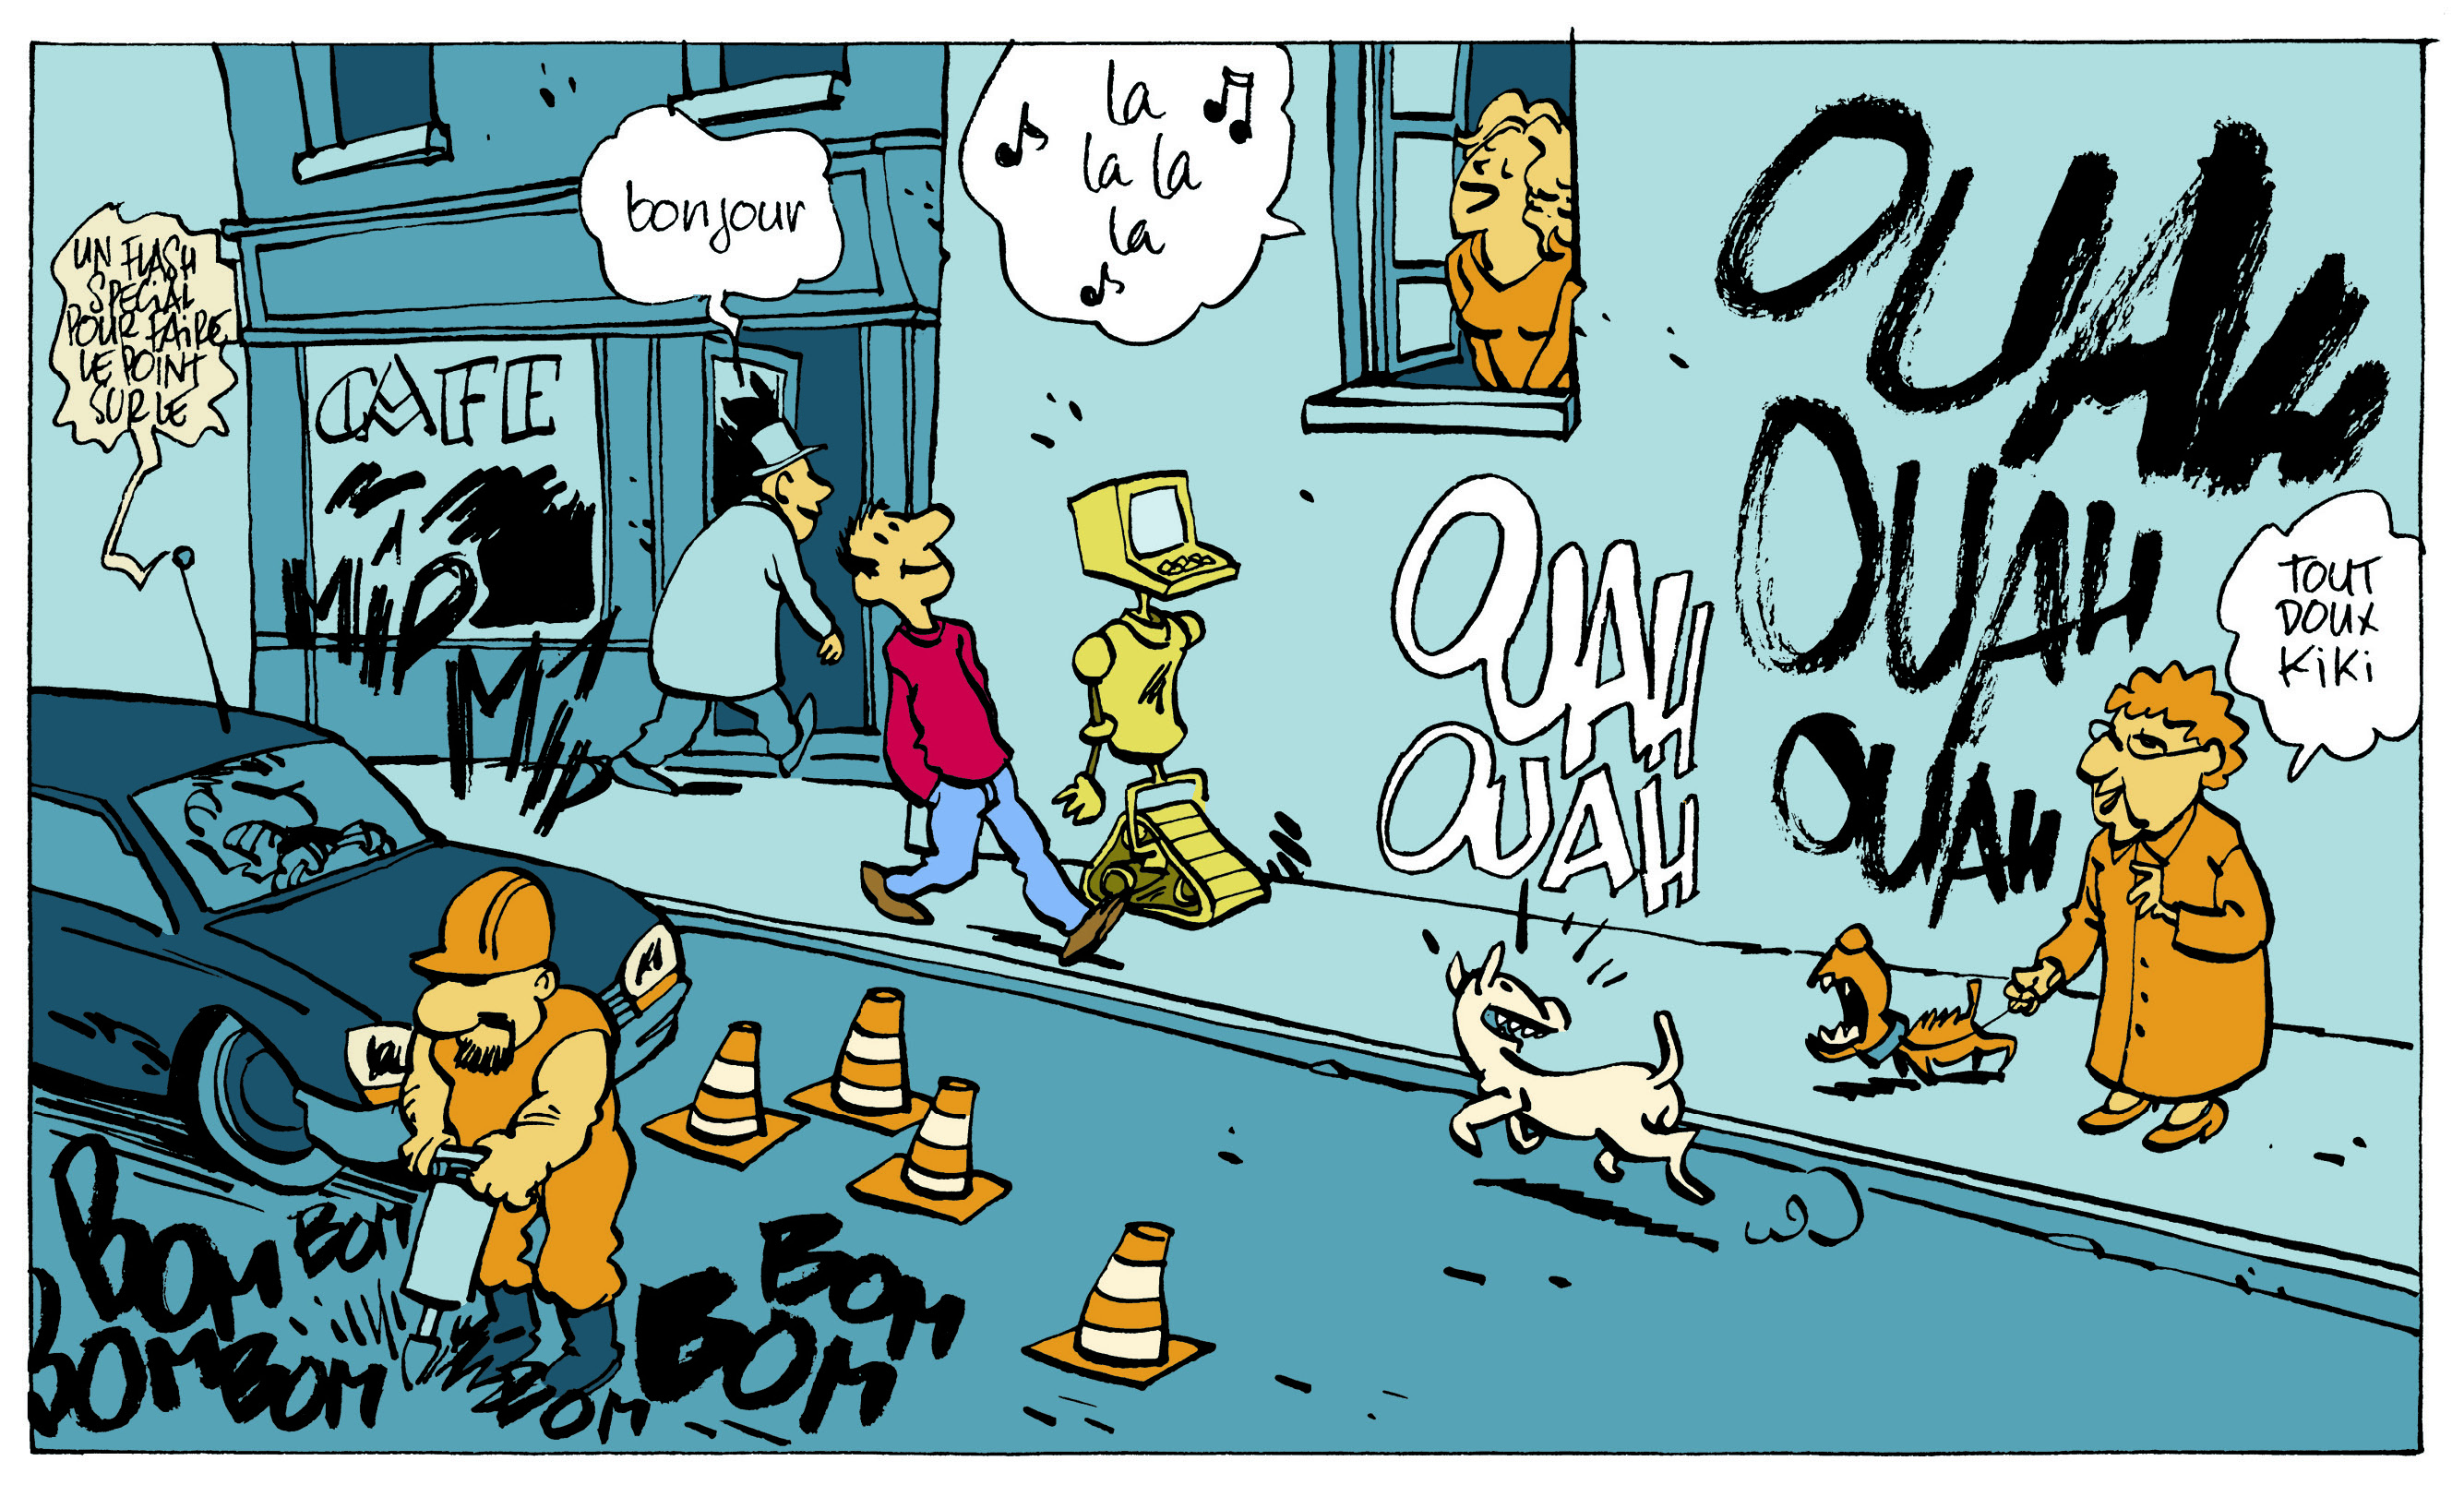
\includegraphics[width=\linewidth]{application/audio_scene.jpg}
%     \end{sidecaption}
% \end{figure}
Recalling the (discrete) time-domain signal model already discussed in~\cref{subsec:processing:mixing}, the signal recorded at the $\idxMic$-th microphones reads
\begin{equation}
    \label{eq:application:mix}
    \mic_\idxMic[n] = \sum_{\idxSrc = 1}^{\numSrcs}
        \kparen{\flt_{\idxMicSrc}( \positionMicrophone_{\idxMic}  | \positionSource_{\idxSrc}) \convDis \src_{\idxSrc}} [n] + \nse_\idxMic[n]
    ,
\end{equation}
or alternatively, using the source spatial image signals,
\begin{equation}
    \label{eq:application:mix_img}
    \begin{aligned}
        \mic_\idxMic[n]     &= \sum_{\idxSrc = 1}^{\numSrcs} \img_{\idxMicSrc}[n] + \nse_\idxMic[n],\\
        \img_{\idxMicSrc}[n]  &= \kparen{\flt_{\idxMicSrc}( \positionMicrophone_{\idxMic}  | \positionSource_{\idxSrc}) \convDis \src_{\idxSrc}}[n]
        .
    \end{aligned}
\end{equation}
Note that the filter $\flt_{\idxMicSrc}(\positionMicrophone_{\idxMic} | \positionSource_{\idxSrc})$ denotes the \RIR/ where we intentionally highlight the dependencies on geometry,
namely, accounting for the whole sound propagation for the source position $\positionSource_{\idxSrc}$ to the microphone position $\positionMicrophone_{\idxMic}$.
In fact, as discussed throughout~\cref{pt:background}, we can decouple the information of indoor microphone natural recordings into two orthogonal contributions:
the \RIRs/ (thus the mixing matrix) accounting for only the sound propagation, and the source signals describes only the semantic content.

\newcommand{\setMicSignals}{\ensuremath{\set{\mic_{\idxMic}}_\idxMic}}
\newcommand{\setSrcSignals}{\ensuremath{\set{\src_{\idxSrc}}_\idxSrc}}
\newcommand{\setSrcPositions}{\ensuremath{\set{\positionSource_{\idxSrc}}_\idxSrc}}
\newcommand{\setFltSignals}{\ensuremath{\set{\flt_{\idxMicSrc}(\positionMicrophone_{\idxMic} | \positionSource_{\idxSrc})}_{\idxMicSrc}}}


\subsection{Problem formulation}
The Audio Scene Analysis Problems presented already in the introductory chapter (See~\cref{sec:intro:scene}) can now be extended and rewritten in terms of the above notation.
Furthermore, we will consider here the only ones directly addressed in this thesis: room impulse response estimation, audio source separation, Spatial filtering, sound source localization, and room geometry estimation.

\begin{table}[!h]

    \begin{fullwidth}
    \centering
    \small
    \renewcommand{\arraystretch}{1.3}

    \begin{tabular*}{\linewidth}{@{\extracolsep{\fill}}lllll@{}}
    \toprule
    Audio scene analysis problems & \textit{from the mixtures $\setMicSignals$, can we estimate...}  & Chapter\\
    \midrule

    Audio Source Separation     & \begin{tabular}[c]{@{}l@{}}the source signals $\setSrcSignals$ and\\ \hspace{1em} the filters $\setFltSignals$?\end{tabular}   & \cref{ch:separake}\\

    Spatial filtering           & \begin{tabular}[c]{@{}l@{}}the source signals $\setSrcSignals$,\\ \hspace{1em} knowing the filters $\setFltSignals$?\end{tabular} & \cref{ch:decharateapp}~\cref{sec:dechorateapp:se}\\

    Sound Source Localization   & the source positions $\setSrcPositions$?                              & \cref{ch:mirage}\\

    Room Geometry Estimation    & the shape of the room?                                                & \cref{ch:decharateapp}~\cref{sec:dechorateapp:rooge}\\
    \bottomrule
\end{tabular*}


% Channel (or \RIR/) Estimation            & the filters $\setFltSignals$ ?                            & \cref{pt:estimation}\\

% Acoustic Echo Retrieval     & the early echoes' timings and gain accounted in $\setFltSignals$ ?     & \cref{pt:estimation}\\

% \RIR/ measurement           & the filters $\setFltSignals$, knowing $\setSrcSignals$ ?               & \cref{ch:dechorate}\\
% Speech Enhancement          & the signal of the $\idxSrc$-th target source $\src_{\idxSrc}$?        & \cref{ch:decharateapp}\\

    % \hline

    \caption{List of audio scene analysis problems considered in this thesis accompanied by their mathematical description.}
    \label{tab:processing:problems}

    \end{fullwidth}

\end{table}

\mynewline
As introduced in~\cref{sec:estimation:problem}, these problems can be said either \textit{informed} or \textit{blind} and the related scenario \textit{active} or \textit{passive}.
These two dichotomies emphasize the amount of prior knowledge available for solving them.
As opposed to the active scenario, where the source signal is known, transmitted, and available, the passive one considers only the microphone measurements.
For instance, when addressing the active echo estimation problem or \RIR/ measurement, the exact time of emission of the source signal is known, as well as the source signal itself.
\\The second dichotomy refers to the possibility of exploiting prior knowledge to solve the problem more easily.
This information may derive from annotations and meta-data.
In the community of audio source separation, the following definitions were proposed in~\citeonly{vincent2014blind}:
as opposed to informed problems, for solving the blind ones, absolutely no information is given about the source signal or the mixing process.
In between, there are \textit{semi-blind} or \textit{guided} problems:
here general information is available, such as on the nature of the source signal (speech, music, environmental sounds),
microphone position, recording scenario (indoor, outdoor, professional music), mixing process, \etc/.
In some books and works other categories of problems are defined, such as \emph{weakly-guided}, \emph{strongly-guided}.
Here we do not consider these distinctions.

\mynewline
In the considered echo-aware applications, the echoes properties build our prior knowledge on the problem.
Therefore, according to the above taxonomy, the addressed problems are necessarily guided.
In general and unless specified, this is the only knowledge we will assume to have.
Based on this, we will now review some classical works for solving the above problems.


\section{Literature overview}\label{sec:application:sota}
Here we present the general overview of the literature related to the problems considered in this thesis: multichannel audio source separation, Spatial filtering, and sound source localization.
We will limit the discussion to the most relevant techniques adopted nowadays with respect to the acoustic propagation modeling.
Later in the thesis, dedicated sections on echo-aware method to address these problems will be provided in each related chapter.
Since room geometry estimation is mainly based on echo estimation and labeling discussed in~\cref{subsec:estimation:active_rir}, its description is postponed to~\cref{sec:dechorateapp:rooge}.


\subsection{On Multichannel sound source separation}\label{subsec:application:separation}
Multichannel audio source separation refers to the process of extracting acoustic signals from multichannel mixtures featuring targets, interfering, and noisy sounds.
In psychoacoustics, this problem is known as \textit{the cocktail party problem}~\citeonly{cherry1953cocktail}, referring to the human ability to focus on a particular stimulus in a audio scene.
This problem has interested mainly in two research fields in the audio signal processing community: speech and music processing.
Both share many methods, which are accordingly modified, taking into account scenarios and applications.
\marginpar{
    \footnotesize\itshape
    Many other methods have been proposed in the literature.
    The reader can refer to \citeonly{vincent2018audio, makino2018audio}
}
In the context of the multichannel speech recordings, some of the most successful and popular methods used nowadays
include Spatial filtering, \TF/ masking, and end-to-end regression.
In this thesis, we deliberately distinguish between the Spatial filtering, which will be discussed in the following subsection, and \TF/ masking.
\\\TF/ masking relies on \TF/ diversity of the sources and processes each mixture channel separately.
In a nutshell, it involves computing the \acp{STFT} of the mixture channels, multiplying them by masks containing gains between 0 and 1.
One of the most popular masking rules is adaptive Wiener filtering.
For each time-frequency bin, the \acp{STFT} of the estimated source spatial images $\IMG_{\idxMicSrc}$ of the $\idxSrc$-th source at the $\idxMic$ microphone, writes
\begin{equation}
        \hat{\IMG}_{\idxMicSrc} = \underbrace{\frac{\powerOf{\IMG_{\idxMicSrc}}}
                                        {\sum_{\idxSrc=0}^\numSrcs \powerOf{\IMG_{\idxMicSrc}}}}
                                        _{\text{Wiener filter}} \; \MIC_\idxMic
\end{equation}
where $\MIC_\idxMic$ is the \STFT/ of the microphone channel. Here the \TF/ bin is omitted for clarity.
\\In order to be computed, the Wiener filter requires estimating all the source spatial images, or equivalently, the mixing filters and the source signals.
Therefore, this approach has been generalized in several ways to account for both these unknowns.
In these thesis we stress the difference between source separation and Spatial filtering.
In the former, all the source signals and mixing filters are indispensable to weigh each of the \TF/ bins of the microphone channel's \STFT/.
As opposed to, in the latter problem, the ``masks'', that is the spatial filters, are estimate only based the mixing filters and noise statistics.
In multichannel recordings, a clear overlap exist between the two problems, and some techniques can be used reciprocally.
Furthermore the related research trends are now converging under the same umbrella of the so-called \textit{speech enhancement}.
The work~\citeonly{gannot2017consolidated} provide an unified framework merging source separation and Spatial filtering.
Nevertheless, we will treat them as separated problems.

\mynewline
Moreover, the benefit of the \TF/ masking approach is that the masks can be estimated in various ways.
For instance, clustering and classification techniques~\citeonly{rickard2007duet} can be used to assign each \TF/-bin to each of the sources.
Recently learning-based methods have been used in this sense on the same task~\citeonly{hershey2016deep,wang2018multi}.
Alternatively, deep learning techniques can used to directly estimated the sources' \TF/, as done in one of the reference implementation~\citeonly{stoter2019open}.
The work of \citeonly{nugraha2016multichannel}, instead, uses a deep learning model build by unfolding the the popular Multichannel \ac{NMF} source separation framework of~\citeonly{ozerov2010multichannel, sawada2013multichannel}.

\mynewline
The Gaussian-based Multichannel \ac{NMF}~\citeonly{ozerov2010multichannel} is one of the most successful framework for source separation using \TF/ masks.
It combines the \ac{NMF} and narrowband spatial model (discussed in ~\cref{subsec:processing:model:stft}) and deploys optimization-based framework for estimating both the mixing matrix and the sources.
One of the main advantage of this approach is that it allows to easily incorporated prior knowledge on the problem.
Thanks to the narrowband approximation (\cref{eq:processing:narrow}), spatial and semantic content are orthogonal and can be treated disjointedly.
This opens to many possibilities, such as, using pre-trained dictionaries to model source content~\citeonly{schmidt2006single, smaragdis2009sparse}, or using proper model for the mixing filters, such as \RIRs/, steering vectors, \ReTFs/, \etc/.

\mynewline
However, it has been shown that even with oracle \TF/~\citeonly{luo2019conv}, the estimation is still affected by artifacts.
This limitation affects all the approaches operating in the \TF/ domain.
To overcome this, end-to-deep deep learning models~\citeonly{luo2019conv, tzinis2020sudo} were developed and now hold the record in source separation.
These models work directly in the time domain: both input and output are time-domain waveforms.
This approach has prove to reach good separation quality, especially in terms of perceived sounds at the listener.
Nevertheless, all deep learning methods rely on trained black-box models for which is hard to inject prior knowledge.
Instead, Multichannel NMF-based frameworks accounts for this freedom.

\newthought{Multichannel NMF source separation methods} can be grouped according to how they model sound propagation of the mixing process:
\begin{itemize}
    \item those that simply ignore it \citeonly{le2015deep};
    \item (\textit{free field propagation}) those that assume a single anechoic path \citeonly{rickard2007duet, nesta2012convolutive} ;
    \item (\textit{reverberant propagation}) those that model the \RTFs/ entirely \citeonly{ozerov2010multichannel, duong2010under, li2019expectation};
    \item (\textit{reverberant propagation}) and those that attempt to separately estimate the contribution of the early echoes and the contribution of the late tail \citeonly{leglaive2015multichannel}.
\end{itemize}
Therefore, these existing approaches either ignore sound propagation or aim at estimating it fully, which affect the quality of the separation.
In the first case, strong echoes and reverberant constitute a low bound in the separation capability.
In fact, these elements of the sound propagation blur and spread the energy of the source source over multiple \TF/ bins, for which the assignation is harder.
When computing the \TF/ masking operation, these bins may introduce strong artifacts.
In the second case, the algorithm need to estimated more parameters with consequences in complexity and estimation accuracy.

\newthought{Echo-aware source separation methods} have been introduced as a possible solution to overcome some of these limitations,.
More details will be given in~\cref{ch:sepakare}, where a new method for speech source separation based on the Multichannel \NMF/ framework and echoes is described.

\subsection{On Spatial filtering}\label{subsec:application:filtering}\marginpar{
    \footnotesize\itshape
    For a comprehensive review on Spatial filtering methods, the reader can refer to the book~\citeonly{VanTrees2004Optimum}.
}
Spatial filtering aim at the enhancement of a desired signal while suppressing the background noise and/or interfering signals.
It is a large and active research field that has interested the signal processing and telecommunication communities since several decades.
It has produced an vast literature including several reference books dedicated to the topic.
For more details in this direction, the reader can refers to, e.g., the book~\citeonly{VanTrees2004Optimum}.
In audio, this topic was been extensively review in the context of speech enhancement in a recent publication~\citeonly{gannot2017consolidated}\sidenote{
    The content of this work has been extended in the book~\citeonly{vincent2018audio}.
}

\mynewline
In Spatial filtering, the \RIRs/ (and related models, \eg/, \RTFs/, steering vectors or \ReTFs/) play a central role.
Intuitively, giving the mixing model in~\cref{eq:application:mix}, the enhancement of a target source can be achieved by merely denoising the recordings and filtering by the inverting \RIRs/.
However, this is not always possible as the inversion of the \RIRs/ is not a straightforward operation.
The work in~\citeonly{neely1979invertibility} discuss explicitly the issues of inverting \RIRs/.
Later, several techniques were investigated, which are sometimes referred to as Room Response \textit{Equalization}~\citeonly{cecchi2018room}.
% First, there is a fundamental trade-off between denoising and filtering capabilities, which are related to the number of degree of freedom imposed by the number of microphones available~\citeonly{VanTrees2004Optimum}
% They can be exhausted by imposing unit- and null-gain directions constraints


\newthought{Beamforming} is one of the most famous techniques used in Spatial filtering.
One of the most famous beamformer is the \ac{DS}.
The intuitive idea behind it is to sum the microphone channels constructively by compensating the time delays between the sound source and the spatially separated microphones.
Thus, the target source signal is enhanced, while noise, interferences, and reverberation being suppressed.
\cref{fig:application:beamformers} illustrate this ideas.
Later, this idea has been extended to Frequency and Time-Frequency processing with direct modeling of the noise sources.
More formally, beamformers design mathematical \textit{optimization criterion}, namely objective function, defining the desired shape of the estimated signal and return a filter to be applied to the microphone recordings.
For instance, one may want to keep a unit gain towards the desired sound source's direction while minimizing the sounds from all the other directions.
The literature on beamformers spans in two directions: different optimization criteria and how to estimate the parameters required by their computation.
We will now elaborate the two directions in turn.
\begin{figure}
    \begin{sidecaption}[]{
        Illustration of the \ac{DS} Beamforming in the time-domain applied to a pulse source signal.
        The delays of the recorded signals at each microphone are compensated.
        By summing the shifted signals, the source signal is enhanced.
        Image courtesy of Robin Scheibler, author of ~\citeonly{scheibler2015raking}.
    }[]
        \centering
        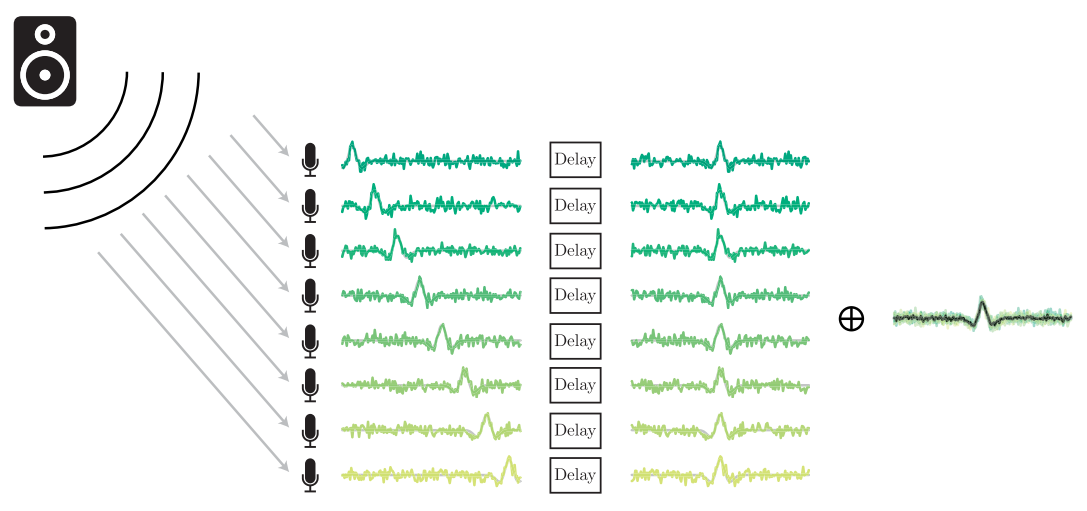
\includegraphics[width=\linewidth]{application/ds.png}
    \end{sidecaption}
\end{figure}

\newthought{Many beamformers criteria} have been proposed.
Among all, some of the most famous are the \DStxt/, the \MVDRtxt/~\citeonly{capon1969high}, the \MaxSNRtxt/~\citeonly{cox1987robust}, the \MaxSINRtxt/~\citeonly{van1988beamforming}, and the \LCMVtxt/~\citeonly{frost1972algorithm}.
These criteria are designed to satisfy different constraints and model prior knowledge, as discussed in~\cref{subsec:dechorateapp:beamformers}.
The reader can also refer to the above-suggested book for more details.

\newthought{Parameter estimation} is a crucial step for beamformers.
We can identify two main categories of parameters: the one related to the \RIRs/ and the one related to the source and noise statistics.
In the former case fall all the methods that model the acoustic propagation of sound.
Therefore, similarly to the methods for separation, we can group existing methods in the following groups:
\begin{itemize}
    \item (\textit{free and far field propagation}) methods based on relative steering vectors build on \DOA/ \citeonly{takao1976adaptive,applebaum1976adaptive,cox1987robust,van1988beamforming};
    \item (\textit{multipath propagation}) methods based on rake rake receiver\citeonly{flanagan1993spatially, Jan1995matched, Dockmanic2015raking, peled2013linearly, scheibler2015raking, Kowalczyk2019raking};
    \item (\textit{reverberant propagation}) methods based on full acoustic channel estimation (see \cref{ch:estimation});
    \item (\textit{reverberant propagation}) methods based on \DOAs/ and the statistical modeling of the diffuse sound field, \citeonly{thiergart2013informed, schwartz2014multi};
    \item (\textit{reverberant propagation}) methods based \ReTF/~\citeonly{gannot2001signal, doclo2002gsvd, cohen2004relative, markovich2009multichannel};
    \item (\textit{reverberant propagation}) methods based on (deep) learning~\citeonly{li2016neural, xiao2016deep, sainath2017multichannel, ernst2018speech};
\end{itemize}
%kodrasi2017evd, markovich2018performance, schwartz2016joint}.
The \acp{DOA}-based methods exploit the closed-form mapping between \DOAs/ and the steering vectors in far-field scenarios.
Thus, good performances are possible only upon a reliable estimation of the \DOAs/ (see next section), a challenging problem in noisy and reverberant environments.
The steering vectors' computation depends on the array geometry, which is unknown in some practical cases.
Alternatively, one can estimate the full acoustic channels, which is a cumbersome task by itself.
\\The \ReTF/-based approaches have been introduced to overcome these two limitations.
They automatically encode the \RIRs/, the geometrical information, and are ``easier'' to estimate than the \RIRs/.
The main limitation of these methods is that they return \textit{spatial source image} at the reference microphone, rather than the ``dry'' source signal.
Therefore, when reverberation is detrimentally affecting the speech signal's intelligibility, post-processing is necessary~\citeonly{schwartz2016joint}.
\\Recently, \ac{DNN} have been proposed for solving this task, either to estimate the beamformer filter~\citeonly{li2016neural directly, xiao2016deep, sainath2017multichannel} or in an end-to-end task~\citeonly{ernst2018speech}
Moreover, \ac{DNN} has been used to estimate some of parameters, such as the \DOAs/~\citeonly{salvati2018exploiting, chazan2019multi}, \ReTF/ estimation~\citeonly{chazan2018dnn}.


\newthought{Early echoes} are neither considered nor modeled as noise terms in the literature discussed thus far.
This direction is taken by the echo-aware methods accounting specifically for the multipath propagation.
We will discuss these methods in more detail in chapter~\cref{ch:dechorateapp} together with their implementation.

\subsection{On Sound Source Localization}\label{subsec:application:localization}
\marginpar{
    \footnotesize\itshape
    The reader can find more details is \SSL/ in the recent review articles
    \citeonly{rascon2017localization,argentieri2015survey}
    as well as in~\citeonly[Chapter 4]{vincent2018audio}.
}
\SSLdef/ consists in determining the distant and direction (or position) of sound sources from microphone (array) in the 3D space, typically in a passive scenario.
As discussed above, the information on the sources' and microphones' position in the room is encoded in the \RIRs/.
Therefore, assuming the uniqueness of the mapping between locations to a \RIR/, it is theoretically possible to retrieve the absolute position of microphones and sources, as show in~\citeonly{ribeiro2010turning, crocco2016estimation}.
However,  this is yet a very challenging task, which typically involves the solution of several sub-problems.
Therefore, it is more common to relax the \SSL/ problem as follows:
First, rather than operating in the  3D cartesian coordinate system, most of the existing methods aim at estimating 2-dimensional \DOAdef/, namely the angles for on the unit sphere with the center in a reference point.
This reference point is usually the center of the microphone array.
This angles are called \textit{azimuth} and \textit{elevation} as shown is~\cref{fig:application:doa}.
Second, they assume far-field scenarios.
The main reasons for adopting such simplifications are the followings:
First, estimating the distance is known to be a much more challenging task than estimating the \DOAs/~\citeonly{vesa2009binaural}.
Second, the task is easier from room geometry estimation, which is more ambitious.
Third, the far-field scenario is a reasonable assumption when using a compact array recording distant sounds.
Finally, in far-field settings, sometimes the only \DOAs/ are sufficient to achieve reasonable speech enhancement performances~\citeonly{gannot2017consolidated}.


\mynewline
Despite these approximations, the \SSL/ problem still challenges today's computational methods, particularly in the presence of reverberation or interfering sources.
Popular approaches for this task consists in two components: \textit{feature extraction} and \textit{mapping}.
First, the audio data are represented as features, as independent as possible from the source's content while preserving spatial information.
Second, the features are mapped to the source position.
Two lines of research have been investigated to obtain such mappings: knowledge-driven and data-driven approaches.

\newthought{Knowledge-based approaches} rely on a physic model for sound propagation \citeonly{knapp1976generalized,stoica1990maximum,dibiase2001robust, dmochowski2007broadband, lebarbenchon2018evaluation}
These models rely on closed-form mapping from the sound's direct path \acl{TDOAs} at the microphone pair and the source's azimuth angle in this pair.
If multiple microphone pairs are available and form a non-linear array, their TDOAs can be aggregated to obtain 2D directions of arrival \citeonly{dibiase2001robust}.
Furthermore, the main difference between these approaches lies in their ability to localize either single sources or multiple ones, their robustness to noise and reverberation, and the particular methods they used.
We can identify the following approaches based on:
\begin{itemize}
    \item subspace methods, such as \MUSIC/~\citeonly{dmochowski2007broadband};
    \item \TDOA/-based techniques, which uses \ac{GCC} functions~\citeonly{knapp1976generalized, Blandin2012, lebarbenchon2018evaluation} to estimate \TDOA/ and then compute the most reliable \DOA/ from them;
    These methods are related to beamforming-based techniques, such as SRP-PHAT\ac{dibiase2001robust}, which search the direction that maximizes the power of the output of a beamformer.
    \item methods based of \RIRs/ estimation and blind system identification ~\citeonly{chen2006time},
    \item methods based on probabilistic framework solved with Maximum Likelihood optimization~\citeonly{stoica1990maximum, laufer2013relative, li2016estimation}.
\end{itemize}
The main limitations of these approaches result in the approximation considered in the models.
In particular, common to all of them is to assumption sound propagation being free-field.
Thus, they intensely suffer in environments it is violated, \eg/, in the presence of strong acoustic echoes and reverberation as discussed as shown in~\citeonly{chen2006time}.

\newthought{Data-driven approaches} have been proposed to overcome the challenging task of modeling sound propagation.
This is done using a supervised-learning framework, that is, using annotated training dataset to implicitly learn the mapping from audio features to source positions~\citeonly{laufer2013relative, deleforge2015acoustic, vesperini2018localizing, chakrabarty2017broadband, adavanne2018direction,  perotin2018crnn, gaultier2017vast}
(to cite a few examples).
Such data can be obtained from annotated real recordings \citeonly{deleforge2015acoustic, nguyen2018autonomous} or using physics-based acoustic simulators \citeonly{laufer2013relative, vesperini2018localizing, adavanne2018direction, chakrabarty2017broadband, perotin2018crnn, gaultier2017vast}.
In comparison to knowledge-driven methods, these methods have the advantage that they can be adapted to different acoustic conditions by including challenging scenarios in the training dataset.
Therefore, these methods were showed to overcome some limitations of the free-field model.
Under this perspective, the data-driven literature can broadly dichotomize into two approaches: end-to-end learning models and two-step models.
In the former case, all the \SSL/ pipeline is encapsulated into a single robust learning framework, taking as input the microphone recordings and returning the source(s) \DOAs/.
Examples of these approaches are the works in~\citeonly{chakrabarty2017broadband, adavanne2018direction}, where the task is performed with \acp{DNN} models.
In the latter, learning models are used as a substitute for either feature extraction or the mapping.
For instance, in~\citeonly{laufer2013relative, deleforge2015acoustic, gaultier2017vast, nguyen2018autonomous}, \acp{GMM}-based models ware used to learning the mapping from features derived from the \ReTF/ of pair of microphones.
In~\citeonly{vesperini2018localizing}, the author proposes to use \ac{NN} models to estimate source location using features computed through \ac{GCC-PHAT}.
Despite the considerable benefit of data-driven approaches in learning complex functions, their main limitation lies in the training data.
First, these data are typically tuned for specific microphone arrays and fail whenever test conditions strongly mismatch training conditions.
Moreover, due to the cumbersome task of collecting building annotated datasets that cover as many possible scenarios as possible, physics-based simulators are used.
Therefore, as they ``learn a model from model'' which, in turn, rely on assumptions, they may not be able to generalize to real-world conditions.


\newthought{To conclude} most of the methods developed for \SSL/, and in particular \DOAs/ estimation, including the above listed, regard reverberation and, in particular, acoustic echoes as a nuisance.
The recent \ac{DNN} based supervised learning approaches have proven to succeed in the presence of harsh acoustic conditions.
However, they are based on black-box, where knowledge about sound propagation is not trivial to inject.
Based on these limitations, we propose to combines the best of the two worlds:
using \ac{DNN} to estimate echoes~\cref{ch:lantern} and use well-understood knowledge-based method to map echoes to source \DOAs/~\cref{ch:mirage}.


\subsection{Room Geometry Estimation}
Since \RooGE/ is manly based on echo estimation and labeling, its discussion is reported in~\cref{subsec:estimation:active_rir, subsec:dechorateapp:rooge}.


\section{Conclusion}\label{sec:application:conclusion}
This chapter presented some fundamental audio signal processing problems and an overview of related approaches to address them.
These problems will be considered in their echo-aware settings in the following chapters.

% Based on this idea, so-called \textit{echo-aware} methods have been introduced few decades ago, where matched filters (or rake receivers) are used to constructively sum the sound reflections \citeonly{Jan1995matched, Affes1997signal} and build beamformers achieving much better sound qualities \citeonly{gannot2001signal}.
% This methods have recently regained interested as manifested by the European project SCENIC~\citeonly{Annibale2011scenic} and the UK research \href{http://www.s3a-spatialaudio.org/}{S$^3$A project}.
% They show that knowing the properties of a few early echoes can boosts performances of typical indoor audio inverse problems such as speech enhancement (SE) \citeonly{Dockmanic2015raking, Kowalczyk2019raking}, sound source localization \citeonly{ribeiro2010turning, DiCarlo2019mirage}, and separation \citeonly{scheibler2017separake, leglaive2016multichannel}.
% Another fervent area of research spanning transversely the audio and acoustic signal processing fields is estimating the room geometry blindly from acoustic signals.
% As presented by Crocco \textit{et al.} in \citeonly{crocco2017uncalibrated}, the end-to-end room geometry estimation (RooGE) involves many subsequent subtasks:
% RIR estimation, peak picking, microphones calibration, echo labeling, reflectors estimation. Acoustic echo retrieval (AER) is common to many of these topics. It consists in estimating the properties of echoes such as their TOAs and energies. The former problem is referred to as TOA estimation, or time-delay estimation when the direct-path is taken as reference. Furthermore, as interesting applications, these methods have been recently used in active scenarios, namely knowing the transmitted signals, using unmanned aerial vehicle (UAV, a.k.a. drones) \citeonly{jensen2019method, Boutin2020drone} and mobile-phones \citeonly{Shih2019phone}.





%% models %%
% \newthoughtpar{end2end \vs/ 2step}
% end2end: from data to (feature to) target
% \\2-step: (from data to features) + features to target

% \newthoughtpar{Knowledge-based \vs/ Learning-based}
% \begin{itemize}
%     \item Bottom-up vs Top-down information processing
%     \item Knowledge-based: specialized signal processing and mathematical algorithms informed by knowledge;
%     \item Learning-based: machine learning usually trained in supervised fashion.
% \end{itemize}
